In this chapter we present our results in chronological order. Many of the results 
are found based on earlier results, so we find it natural to include some amount 
of discussion of the results as they are presented to be able to argue for why we 
approach the problem the way we do further down.
\section{CAMELS-GB}
\subsection{Feature selection}
Note that when doing model selection we do not look at test set performance, only 
performance on the cross validated train set.
%\begin{table}
%    \begin{adjustbox}{width=\textwidth}
%    \begin{tabular}{lr}
\toprule
{} &     Coeff \\
\midrule
Q95                   &  1.211018 \\
elev\_50               &  0.464968 \\
conductivity\_cosby\_50 &  0.443736 \\
intercept             &  0.443277 \\
porosity\_cosby\_50     &  0.409635 \\
conductivity\_hypres\_5 &  0.257509 \\
high\_prec\_dur         &  0.211253 \\
gauge\_easting         & -0.211231 \\
tawc                  & -0.326509 \\
elev\_max              & -0.349975 \\
conductivity\_cosby\_5  & -0.351292 \\
baseflow\_index\_ceh    & -0.417237 \\
bares\_perc            & -0.463398 \\
elev\_10               & -0.496951 \\
conductivity\_cosby\_95 & -0.839606 \\
porosity\_hypres\_5     & -1.030274 \\
low\_prec\_freq         & -1.055273 \\
dwood\_perc            & -1.288324 \\
p\_mean                & -2.015090 \\
ewood\_perc            & -2.146395 \\
urban\_perc            & -2.332153 \\
shrub\_perc            & -3.735298 \\
grass\_perc            & -4.010000 \\
crop\_perc             & -4.868455 \\
\bottomrule
\end{tabular}


%    \end{adjustbox}
%    \caption{Table for attempt at linear regression. This model is fit on the static
%    features as input values, and the NSE of an LSTM trained without static features
%    for each basin in the validation set. The $R^2$ score of this model is $\approx 0.5$}
%    \label{linreg_no_static_table}
%\end{table}
%In table \ref{linreg_no_static_table} we can see that our linear regression used to model 
%the relationship between NSE value of models and static features has decided that 
%several features are important. All these coefficients have a p-value $<0.5$. The 
%problem with this model was that it achieved an $R^2$ score of $\approx 0.5$, meaning 
%it does not actually explain the relationship well. We therefore choose to change 
%strategy for feature selection. 
\begin{figure}
    \includegraphics{{correlation_reduction/all_features/corr_and_dendrogram}.pdf}
    \caption{The Pearson correlation matrix and the corresponding hierarchial
    cluster of the training set before removing correlated features. The process
    of creating the dendrogram is described in chapter \ref{Feature selection}. 
    For readability's sake we cannot include every label in the correlation matrix.}
    \label{corr_matrix_full}
\end{figure}

\begin{figure}
    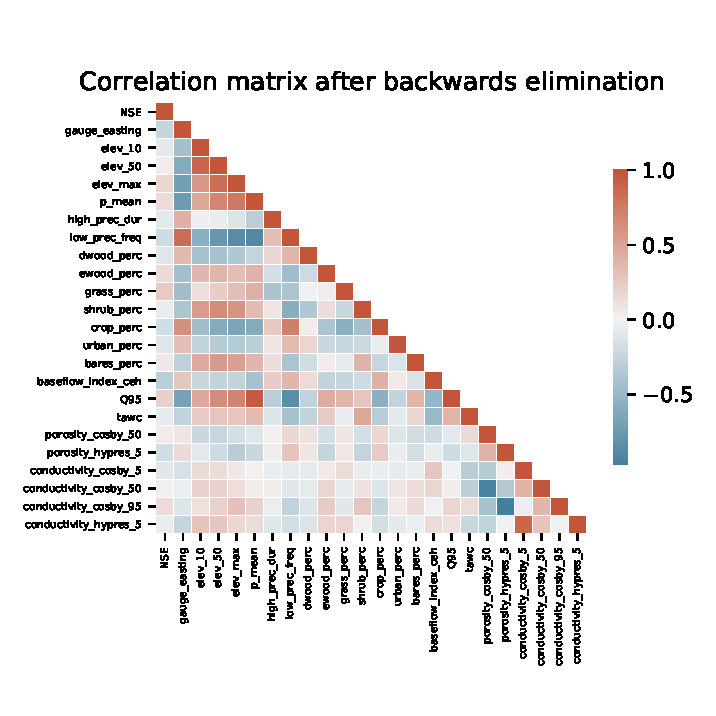
\includegraphics{reduced_matrix.pdf}
    \caption{Correlation matrix after backward selection}
    \label{corr_matrix_reduced}
\end{figure}

\subsection{Performance of full model}
\begin{figure}
%\includegraphics[scale=1]{{permutation/all_features_cv/histogram_all}.pdf}
    \includegraphics{{figures/permutation/all_features_cv/histogram_all}.pdf}
\caption{The two most important (above) and least important (below) features according 
to the permutation test}
\label{Hist all}
\end{figure}



\begin{table}
    \begin{adjustbox}{width=\textwidth}
    \begin{tabular}{l|l}
\toprule
Camels-US &     Camels-GB \\
\midrule
time series: & \\
\midrule
prcp$($mm$/$day$)$ $[$mm$/$day$]$ & precipitation [mm/day] \\
    $\frac{\text{tmax} + \text{tmin}}{2}$ [K] & temperature [K]\\
    srad(W/m2) [W$/$m$^2$] & shortwave\_rad [W$/$m$^2$] \\
\midrule
    attributes: & \\
\midrule
elev\_mean [m]  & elev\_mean [m] \\
area\_gages2 [km$^2$] & area [km$^2$] \\
p\_mean [mm/day] & p\_mean [mm/day] \\
    pet\_mean [mm/day] & pet\_mean [mm/day] \\
p\_seasonility & p\_seasonality \\
frac\_snow & frac\_snow \\
    high\_prec\_freq [days / yr] & high\_prec\_freq [days / yr] \\
    high\_prec\_dur [days] & high\_pref\_dur [days]  \\
    low\_prec\_freq [days / yr] & low\_prec\_freq [days / yr] \\
    low\_prec\_dur [days] & low\_prec\_dur [days] \\
aridity & aridity \\
forest\_frac & dwood\_frac + ewood\_frac \\ 
root\_depth\_50 [m] & root\_depth\_50 [m] \\
soil\_depth\_pelletier [m] & soil\_depth\_pelletier [m] \\
soil\_porosity & porosity\_cosby \\
soil\_conductivity [cm/h] & conductivity\_cosby [cm/h] \\
sand\_frac & sand\_perc  / 100 \\
silt\_frac & silt\_perc / 100 \\ 
clay\_frac & clay\_perc  / 100 \\ 
organic\_frac & organic\_perc / 100 \\
    gvf\_max & $1 -\frac{\text{urban\_perc}+\text{inwater\_perc}}{100} $ \\
\bottomrule
\end{tabular}


    \end{adjustbox}
    \caption{Common features}
    \label{Common features}
\end{table}

\begin{figure}
    \centering
    \includegraphics{{CDFs/mixed_model_comparisons}.pdf}
    \caption{top kjeks}
    \label{main cdf}
\end{figure}
